\documentclass[conference]{IEEEtran}
\IEEEoverridecommandlockouts
% The preceding line is only needed to identify funding in the first footnote. If that is unneeded, please comment it out.
\usepackage{cite}
\usepackage{amsmath,amssymb,amsfonts}
\usepackage{graphicx}
\usepackage{textcomp}
\usepackage{xcolor}
\usepackage{algorithm}
\usepackage{algpseudocode}
\algnewcommand\algorithmicinput{\textbf{Input:}}
\algnewcommand\INPUT{\item[\algorithmicinput]}
\algnewcommand\algorithmicoutput{\textbf{Output:}}
\algnewcommand\OUTPUT{\item[\algorithmicinput]}


\def\BibTeX{{\rm B\kern-.05em{\sc i\kern-.025em b}\kern-.08em
    T\kern-.1667em\lower.7ex\hbox{E}\kern-.125emX}}
\begin{document}

\title{Aperiodic Scheduling of Real Time Tasks in Cloud Environment\\}

\author{\IEEEauthorblockN{Sahil Kumar Sahu}
\IEEEauthorblockA{\textit{Computer Science Engineering)} \\
\textit{College Of Engineering and Technology}\\
Bhubaneswar, India \\
sahilsahu19970@gmail.com}
\and
\IEEEauthorblockN{Tanmay Kumar Rath}
\IEEEauthorblockA{\textit{Computer Science Engineering} \\
\textit{College Of Engineering and Technology}\\
Bhubaneswar, India \\
tanmayrath98@gmail.com}

}

\maketitle

\begin{abstract}
 A real-time system consists of both aperiodic and periodic tasks. Periodic tasks have regular arrival
times and hard deadlines. Aperiodic tasks have irregular arrival times and either soft or hard deadlines. In this
article, we present three new algorithms, BestFit, FirstFit, and HEFT where task are prioritised according to Deadline and Size which greatly improves Average response times for
soft deadline aperiodic tasks and can guarantee hard deadlines aperiodic tasks. The operation of the the above algorithms, its performance, and schedulability analysis are discussed and compared with previously published aperiodic service algorithms
\end{abstract}

%\begin{IEEEkeywords}
%component, formatting, style, styling, insert
%\end{IEEEkeywords}

\section{Introduction}
THE cloud, consisting of a collection of interconnected and
virtualized computers dynamically provisioned as one
or more unified computing resource(s), has become a revolutionary
paradigm by enabling on-demand provisioning of
applications, platforms, or computing resources for customers
based on a “pay-as-you-go” model [1]. Nowadays, an
increasing number of enterprises and governments have
deployed their applications including commercial business
and scientific research in clouds motivated by the reasonable
price as they are offered in economy of scale, and shifting
responsibility of maintenance, backups, and license management
to cloud providers [2]. Hence, some IT companies are
significantly benefited from cloud providers by relieving
them from the necessity in setting up basic hardware and
software infrastructures, enabling more attention to the
innovation and development for their main pursuit [3].\\[10pt]
\space Real-time systems are used to control physical processes that range in complexity from
auto-mobile ignition systems to controllers for flight systems and nuclear power plants. In
these systems, the correctness of system functions depends upon not only the results of
computation but also on the times at which results are produced.
A real-time task is generally placed into one of four categories based upon its arrival
pattern and its deadline. If meeting a given task's deadline is critical to the system's operation,
then the task's deadline is considered to be hard. If it is desirable to meet a task's
deadline but occasionally missing the deadline can be tolerated, then the deadline is considered
to be soft. Tasks with regular arrival times are called periodic tasks. A common
use of periodic tasks is to process sensor data and update the current state of the real-time
system on a regular basis. Periodic tasks, typically used in control and signal-processing
applications, have hard deadlines. Tasks with irregular arrival times are aperiodic tasks.
Aperiodic tasks are used to handle the processing requirements of random events such as
operator requests. An aperiodic task typically has a soft deadline. Aperiodic tasks that have
hard deadlines are called sporadic tasks. We assume that each task has a known worst-case
execution time. A periodic task has a regular inter-arrival time equal
to its period and a deadline that coincides with the end of its current period. Periodic
tasks usually have hard deadlines, but in some applications the deadlines can be soft.
Soft deadline aperiodic tasks. An aperiodic task is a stream of jobs arriving at irregular
intervals. Soft deadline aperiodic tasks typically require a fast average response time.
Sporadic tasks. A sporadic task is an aperiodic task with a hard deadline and a minimum
inter-arrival time (Mok 1983). Note that without a minimum inter-arrival time restriction,
it is impossible to guarantee that a sporadic task's deadline would always be met.
To meet the timing constraints of the system, a scheduler must coordinate the use of
all system resources using a set of well-understood real-time scheduling algorithms that
meet the following objectives:
Guarantee that tasks with hard timing constraints will always meet their deadlines.
Attain a high degree of schedulable utilization for hard deadline tasks (periodic and sporadic
tasks). Schedulable utilization is the degree of resource utilization at or below which
all hard deadlines can be guaranteed. The schedulable utilization attainable by an algorithm
is a measure of the algorithm's utility: the higher the schedulable utilization, the more applicable the algorithm is for a range of real-time systems. Provide fast average response times for tasks with soft deadlines (aperiodic tasks). Ensure scheduling stability under transient overload. In some applications, such as radar tracking, an overload situation can develop in which the computation requirements of the system exceed the schedulable resource utilization. A scheduler is said to be stable if during overload it can guarantee the deadlines of critical tasks even though it is impossible to meet all task deadlines. The quality of a scheduling algorithm for real-time systems is judged by how well the algorithm meets these objectives. This article develops advanced algorithms to schedule aperiodic tasks. For soft deadline aperiodic tasks, the goal is to provide fast average response times. For hard deadlines aperiodic tasks (sporadic tasks), the goal is to guarantee that their deadlines will always be met. The new algorithm presented here meet both of these goals and are still able to guarantee the deadlines of hard deadline periodic tasks. For simplicity, we assume that periodic tasks have hard deadlines and constant execution times. 1 In Section 2 we review related work on scheduling periodic and aperiodic tasks. Section 3 This section addresses the schedulability of the algorithms and compares its performance with each other. Finally, Section 5 presents a summary and conclusions.  

\section{Related Work}


The researchers [4] have described a fault-tolerant
framework for optimization of resource utilization assuring
availability and responsiveness. They have also designed
pluggable framework for plugging VM replica deployment
algorithms and a real-time publish/subscribe framework for
real-time applications. This paper [5] compared EDF (Earliest
deadline first) and RM (rate monotonic) algorithms. Their
study shows that EDF allows full processor utilization, efficient
use of computational resources and better responsiveness aperiodic activities. This property of EDF makes it
suitable for embedded system where computational resources
are limited and multimedia system where quality of service is
controlled by resource reservation mechanisms. In comparison
to EDF, RM is simpler to implement and applicable to only
high priority task. The writers [6] have identified the technical
challenges for supporting soft real time applications such as
online video streaming, cloud-based gaming, and telecommunication
management in cloud environment. Their survey
displays the recent advancement in the field of real-time virtualization
and cloud computing technology for implementation
of cloud-based real-time applications. This paper [7] showed
Clairvoyant EDF (CEDF) algorithm to insert idle-times for
non-preemptive task. Their simulation results show that CEDF
is better than EDF. The reviewers [8] have used profit time utility
function an d penalty time utility function for modeling of
real-time activities in cloud computing. There is a reward for
early completion and a penalty for deadline misses of real
time tasks. Several experiments conducted display that the
proposed algorithm is better than the traditional EDF approach,
the traditional single time utility function approach, and an
earlier heuristic approach for homogeneous profit/penalty task
model. The researchers [9] proposed a scheduling algorithm for the
improvement of deadline guarantee and resource utilization by
modifying the conservative backfilling algorithm by utilizing
the earliest dead-line first (EDF) algorithm and the largest
weight first (LWF) algorithm in the cloud data center. The
writers of [10] proposed an online-scheduling strategy with
goal to meet the deadline constraint at a lower price for scientific
workflows on hybrid clouds.In our paper Six algorithms are proposed FFE (First Fit EDF), BFE (Best Fit EDF), HEFT (with Priority constraint as 'Deadline' for task selection) and FF (First Fit), BF (Best Fit), HEFT (with Priority constraint as 'Size and Deadline' for task selection) for Aperiodic tasks.


\section{Scheduling Model}
\begin{figure}[htbp]
%\centerline{}
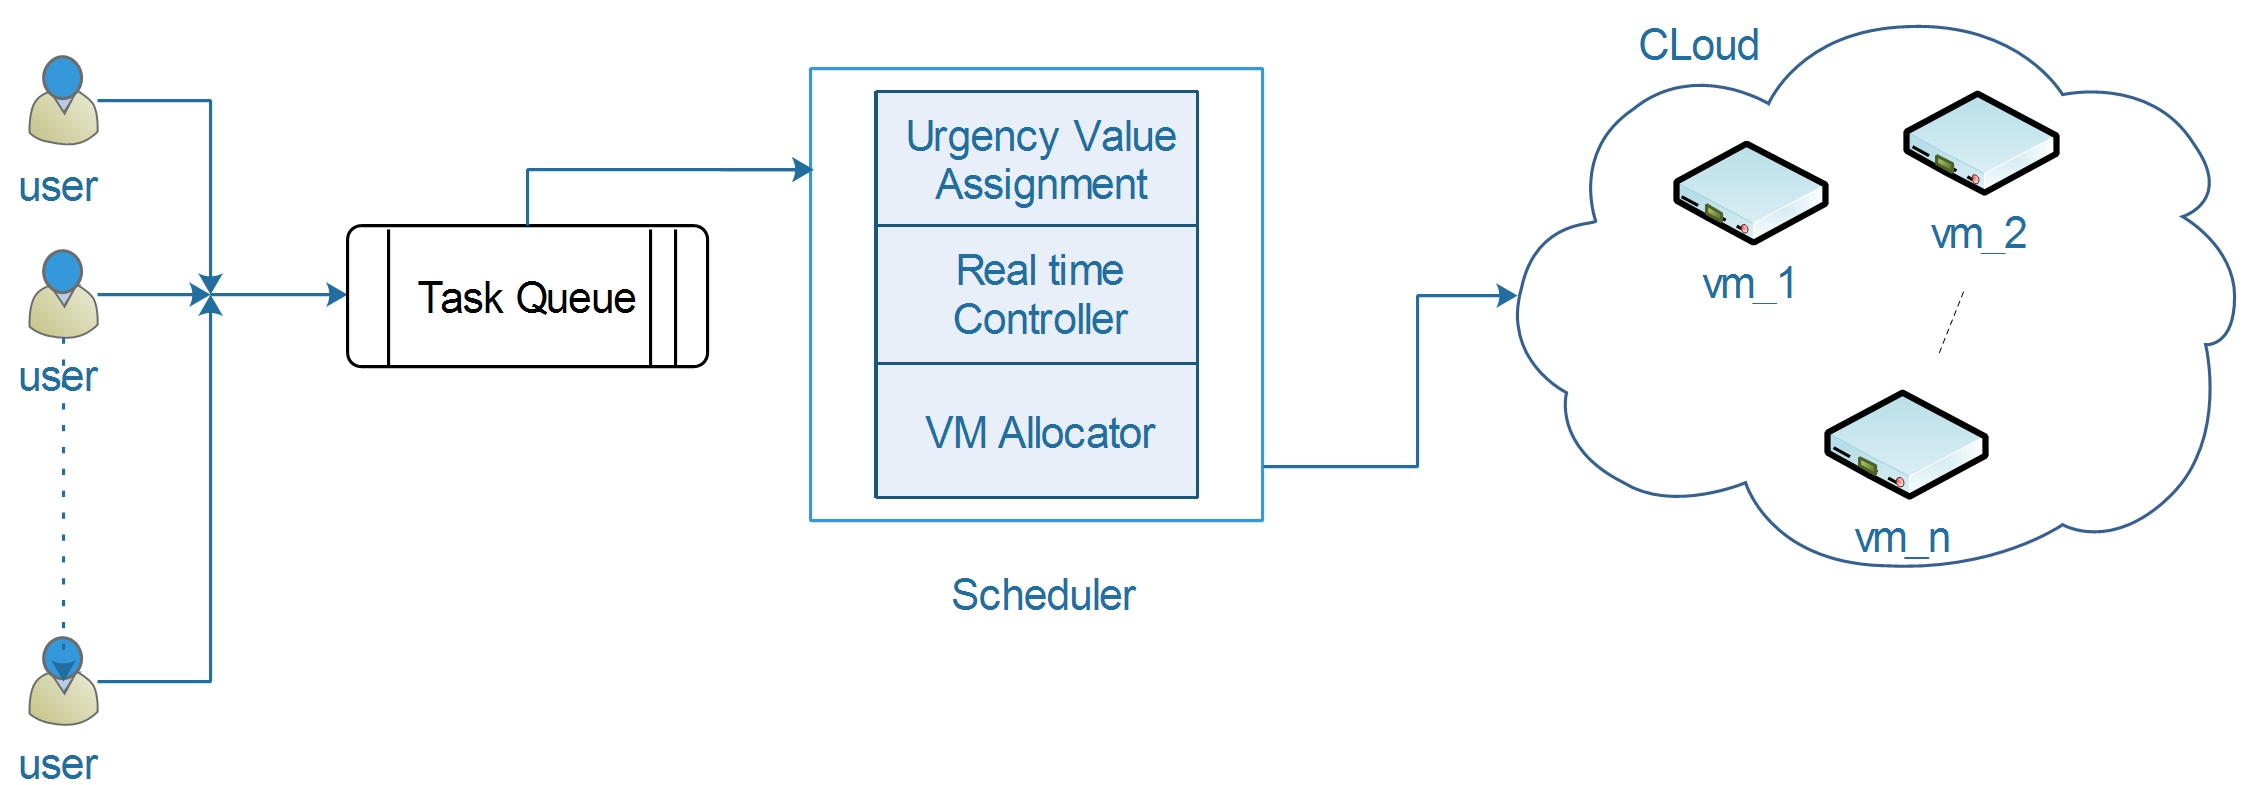
\includegraphics[scale=0.5]{model.jpg}
\caption{Scheduling Model}
\label{fig}
\end{figure}
Target system is characterized by a finite set of
virtual machines (VMs) $V_1, V_2, V_3, ... V_k$. Each VM in VM set V has ready queue to hold executing task, new task and waiting task to be executed. The tasks submitted by different users are stored in ready queue. The Central scheduler consists of ready queue, real-time controller, VM controller. The real-time controller checks whether task will completes its execution before deadline. If not then it informs VM controller, which adds VMs so that task can be completed within timing constraints otherwise task will be rejected. Fig. 1 illustrates the scheduling architecture of the system.\\

\begin{center}
    \begin{tabular}{| l | l | l |}
    \hline
    Sl & Notation & Description \\ \hline
    1 & $nvm_k$ & Total Number Of Vm's in VM set $V_k$\\ \hline
    2 & nt & Total Number Of Tasks. \\ \hline
    3 & $n\_dl_k$ & No of task meeting deadline for VM set $V_k$\\\hline
    4 & $a_i$ & Task Arrival Time. \\ \hline
    5 & $dl_i$ & Task deadline. \\ \hline
    6 & $sz_i$ & Task size. \\ \hline
    7 & $st_{ij}$ & Starting Time of task $t_i$ on Vm $v_j$. \\
    \hline
    8 & $et_{ij}$ & Execution Time of task $t_i$ on Vm $v_j$. \\ \hline
    9 & $ft_{ij}$ & Finish Time of task $t_i$ on Vm $v_j$. \\ \hline
    10 & $|n\_dl/nt|$ or gr & Guuarantee Ratio. \\ \hline
    11 & $|n\_dl|$ or tp & Through Put. \\ \hline
    12 & art & Average Response Time. \\
    \hline
    \end{tabular}
\end{center}

\vspace{10pt}For each virtual machine $v_j$ its CPU performance as $vm\_speed_j$ is measured in terms of number of instructions per second(NIPs), vm's being generated dynamically.\\

Now let $T =\{t_1,t_2,t_3, ...\}$ be set of independent tasks that arrive dynamically. The task $t_i$ having parameter $t_i =\{a_i,sz_i,dl_i\}$, where $a_i$ is the arrival time, $sz_i$ is the size, $dl_i$ is the deadline.


\begin{equation}\label{et}
et_{ij} = \frac{sz_i}{vm\_speed_j}
\end{equation}

\begin{equation}\label{ft}
ft_{ij} = st_{ij}+et_{ij}
\end{equation}
\begin{equation}
cost\_vm_j = k+(vm\_speed_j*c)
\end{equation}
\begin{equation}\label{EST1}
EST_1 = \left(\frac{cost\_vm_j-cost\_vm_min}{cost\_vm_max-cost\_vm_min}\right)
\end{equation}
\begin{equation}\label{EST2}
EST_2 = \left(\frac{et_j-et_min}{et_max-et_min}\right)
\end{equation}
\begin{equation}\label{EST}
EST_{ij} = \theta*EST_1+(1-\theta)*EST_2
\end{equation}
\begin{equation}\label{Pr1}
Pr_1 = \left(\frac{sz_i-sz_min}{sz_max-sz_min}\right)
\end{equation}
\begin{equation}\label{Pr2}
Pr_2 = \left(\frac{dl_i-dl_min}{dl_max-dl_min}\right)
\end{equation}
\begin{equation}\label{Pr}
Pr_i = \theta*Pr_1+(1-\theta)*Pr_2
\end{equation}


Following steps are taken for scheduling a task stored in ready queue
\vspace{10pt}
\begin{enumerate}
\item Tasks are sorted according to their deadlines in three algorithms and according to their size and deadline in rest three algorithms.
\item Scheduler checks the status  VMs such
as running tasks remaining execution time, the information
of tasks in waiting pool including their deadlines, currently
allocated VMs, start time, etc.
\item When a task in ready queue is ready to execute by satisfying the constraints, it is
assigned to respective VM.
\item After the completion of the task, VM becomes free to
accept new task.
\item If a task misses its deadline then it is rejected by the
scheduler.
\end{enumerate}



\section{Scheduling Algorithms}\vspace{30pt}

\begin{algorithm}[h]
\caption{: Pseudo code of $MatrixGeneration()$}
\label{alg1}
\begin{algorithmic}[1]
   \For { each task $t_i$ in $T$}
     \For { each VM $v_j$ in $V$}
      \State  Calculate $et_{ij}$ using Equation \ref{et};
  %   \State  Set $p_i^j=\frac{1}{m}$;
     \EndFor
     \EndFor
\end{algorithmic}
\end{algorithm}

\vspace{30pt}

\begin{algorithm}[]
\caption{: First-Fit based on deadline and size}
\label{euclid}
\hspace*{\algorithmicindent} \textbf{Input: no of task, inter-arrival time} \\
 \hspace*{\algorithmicindent} \textbf{Output: no of task meeting the deadline} 
\begin{algorithmic}[1]
  
\For{$each ~vm~ in~ V$}
   \State Sort task according to size and deadline in ascending order using Equation \ref{Pr}
   \State Generate $et$ matrix using $MatrixGeneration()$
     \For {$i=1$ to $no ~of~ task$}
      \If{$ft_{ij} < dl_i$}
       \For {$j=1$ to no\_of\_vm satisfying constraint} 
          \State Assign task to first Vm.
               \If{vm is busy}
                  \State Increment n\_dl
                  \State break;
                  \Else
                  \State continue;
               \EndIf
       \EndFor
      \EndIf 
    \EndFor  
\EndFor
\end{algorithmic}
\end{algorithm}

\vspace{30pt}

\begin{algorithm}
\caption{: Best-Fit based on deadline and size}
\label{euclid}
\hspace*{\algorithmicindent} \textbf{Input: no of task, inter-arrival time} \\
 \hspace*{\algorithmicindent} \textbf{Output: no of task meeting the deadline} 
\begin{algorithmic}[1]
  
\For{$each ~vm~ in~ V$}
   \State Sort task according to size and deadlines in ascending order using Equation \ref{Pr}.
   \State Generate $et$ matrix using $MatrixGeneration()$
   \State Generate the EST matrix using Equation \ref{EST}
   \State Sort the EST matrix in ascending order, correspondingly Sort $et$ matrix
     \For {$i=1$ to $no ~of~ task$}
      \If{$ft_{ij} < dl_i$}
       \For {$j=1$ to no\_of\_vm satisfying constraint}
          \State Minimize EST and assign task to Vm that satisfies it.
               \If{vm is busy}
                  \State Increment n\_dl
                  \State break;
                  \Else
                  \State continue;
               \EndIf
       \EndFor
      \EndIf
    \EndFor   
\EndFor
\end{algorithmic}
\end{algorithm}

\vspace{30pt}

\begin{algorithm}
\caption{: HEFT based on deadline and size}
\label{euclid}
\hspace*{\algorithmicindent} \textbf{Input:} \\
 \hspace*{\algorithmicindent} \textbf{Output:} 
\begin{algorithmic}[1]
  
\For{$each ~vm~ in~ V$}
   \State Sort task according to size and deadlines in ascending order using Equation \ref{Pr}
   \State Generate $et$ matrix using $MatrixGeneration()$
    \For {$i=1$ to $no ~of~ task$}
      \If{$ft_{ij} < dl_i$}
       \For {$j=1$ to no\_of\_vm satisfying constraint} 
          \State Calculate the finish time for selected Vm's.
          \EndFor
          \EndIf
          \EndFor
          
     \For {$i=1$ to $no ~of~ task$}
      \If{$ft_{ij}$ $<$ $dl_i$}
       \For {$j=1$ to no\_of\_vm satisfying constraint} 
          \State Assign task to Vm with minimum Finish Time.
               \If{vm is busy}
                  \State Increment n\_dl
                  \State break;
                  \Else
                  \State continue;
               \EndIf
       \EndFor
      \EndIf
    \EndFor   
\EndFor
\end{algorithmic}
\end{algorithm}



%\vspace{13cm}
\section{Simulation Result}

Simulation of above system is done in MATLAB R2014b.
Before doing simulation following assumptions are made
Assumptions:
\begin{enumerate}
\item For Fixed no of Task and by varying no of VM's
	\begin{enumerate}
	\item $no~of~task's~=~800$.
	\item $no~of~Vm's$ in range [20,40] with 5 difference.
	\item Size of tasks(NIs) in range [100,10000].
	\item Computation Power of VMs(NIPs) in range [1000,2000].
	\end{enumerate}
\item For Fixed no of Vm's and by varying no of tasks.
	\begin{enumerate}
	\item $no~of~Vm's~=~40$.
	\item $no~of~Task's$ in range [500,1100] with 150 difference.
	\item Size of tasks(NIs) in range [100,10000].
	\item Computation Power of VMs(NIPs) in range [1000,2000].
	\end{enumerate}
\item For Fixed no of Vm's and Taks and by varying Arrival Time.
	\begin{enumerate}
	\item $no~of~Vm's~=~30$.
	\item $no~of~Task's~=~1000$.
	\item Arrival Time in range [0.6,1.2] with 0.2 difference.
	\item Size of tasks(NIs) in range [100,10000].
	\item Computation Power of VMs(NIPs) in range [1000,2000].
	\end{enumerate}
\end{enumerate}
 
Fig. 2 to Fig. 4 are for CASE 1 which shows the result for six algorithms with fixed task by varying no of Vm's. It can observed that the \textbf{average response time} is minimun in case of algorithm's using Deadline and Size for prioritising the tasks therefore are better as compared to (BFE,FFE and HEFT(deadline based)) though it can be noticed that the Guarantee  Ratio is lower. Guarantee Ratio can be ignored as there is not much difference. Similarly in Case 2 and Case 3 whose results are shown in Fig. 5 to Fig. 10 similar phenomenon can be observed.


\begin{figure}[htbp]
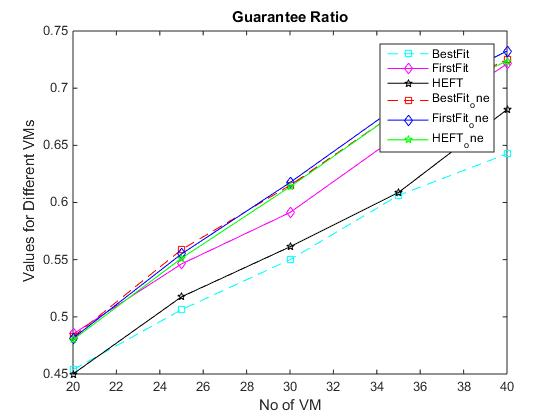
\includegraphics[scale=0.45]{gr_1_p.jpg}
\caption{GR1}
\label{fig}
\end{figure}

%\begin{figure}[htbp]
%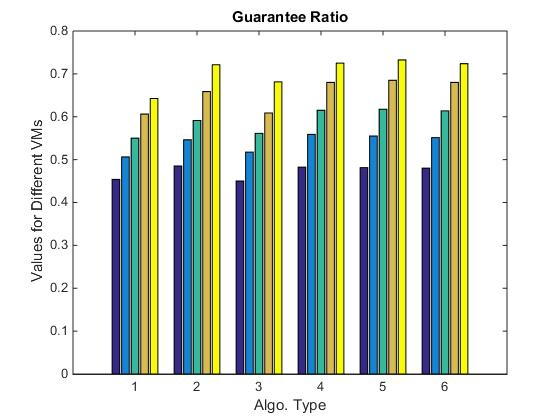
\includegraphics[scale=0.45]{gr_1_b.jpg}
%\caption{GR1}
%\label{fig}
%\end{figure}

\begin{figure}[htbp]
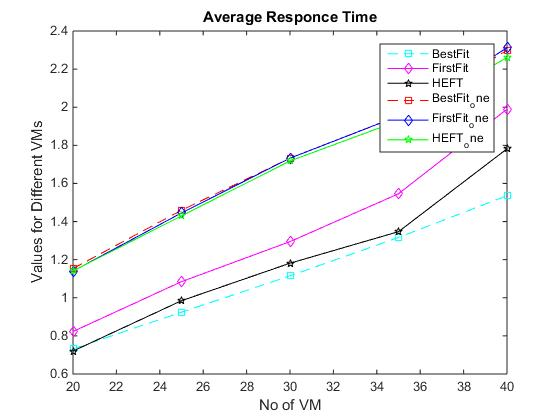
\includegraphics[scale=0.45]{art_1_p.jpg}
\caption{ART1}
\label{fig}
\end{figure}

\vspace{30pt}

%\begin{figure}[htbp]
%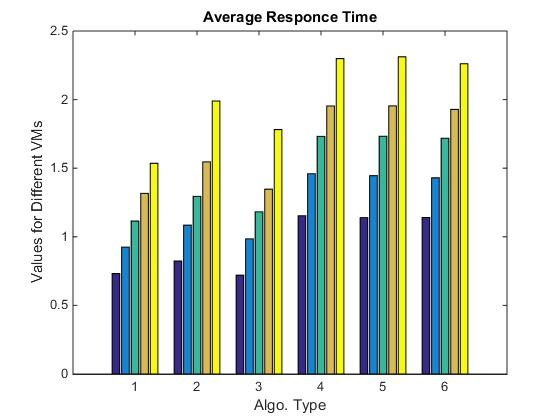
\includegraphics[scale=0.45]{art_1_b.jpg}
%\caption{ART1}
%\label{fig}
%\end{figure}

\begin{figure}[htbp]
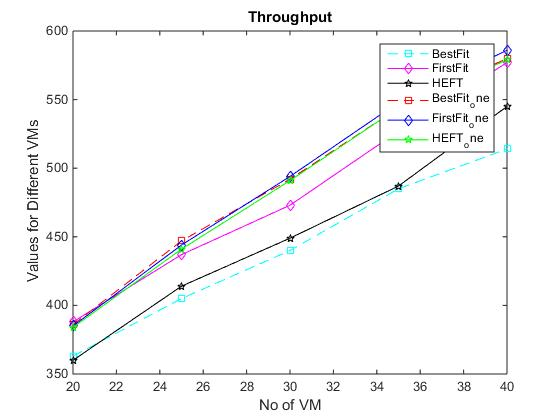
\includegraphics[scale=0.45]{tp_1_p.jpg}
\caption{TP1}
\label{fig}
\end{figure}

%\begin{figure}[htbp]
%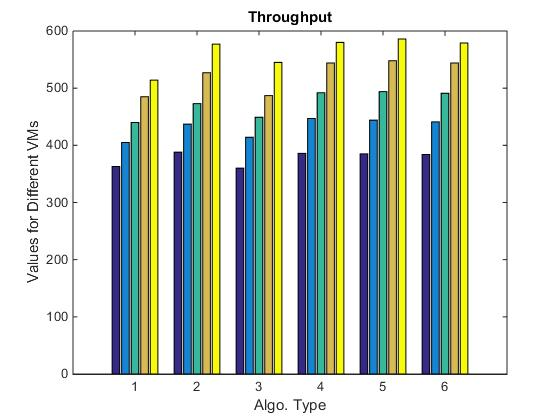
\includegraphics[scale=0.45]{tp_1_b.jpg}
%\caption{TP1}
%\label{fig}
%\end{figure}

\begin{figure}[htbp]
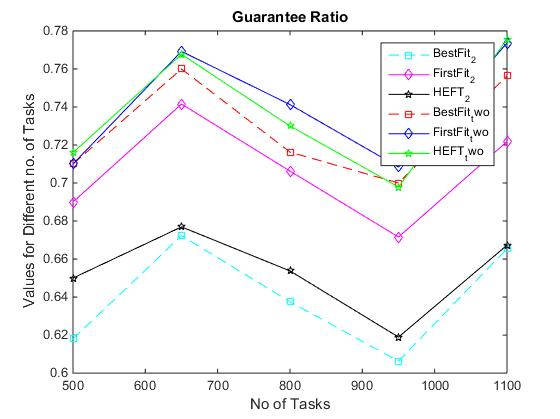
\includegraphics[scale=0.45]{gr_2_p.jpg}
\caption{GR2}
\label{fig}
\end{figure}

%\begin{figure}[htbp]
%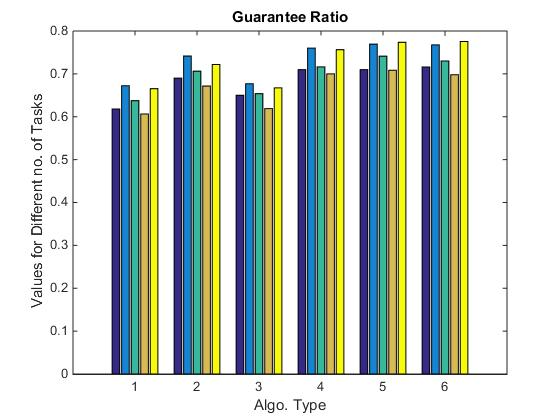
\includegraphics[scale=0.45]{gr_2_b.jpg}
%\caption{GR2}
%\label{fig}
%\end{figure}

\begin{figure}[htbp]
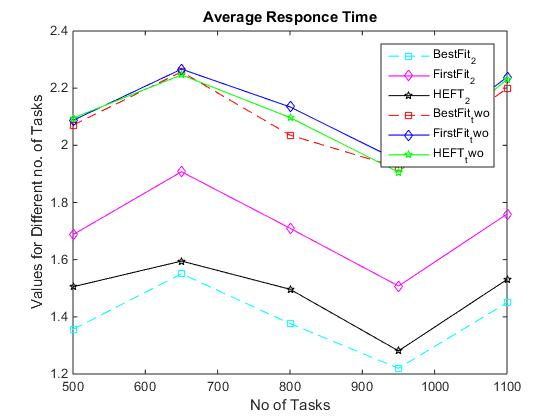
\includegraphics[scale=0.45]{art_2_p.jpg}
\caption{ART2}
\label{fig}
\end{figure}

%\begin{figure}[htbp]
%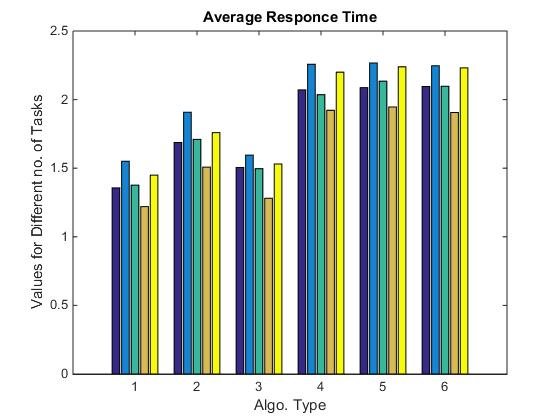
\includegraphics[scale=0.45]{art_2_b.jpg}
%\caption{ART2}
%\label{fig}
%\end{figure}

\begin{figure}[htbp]
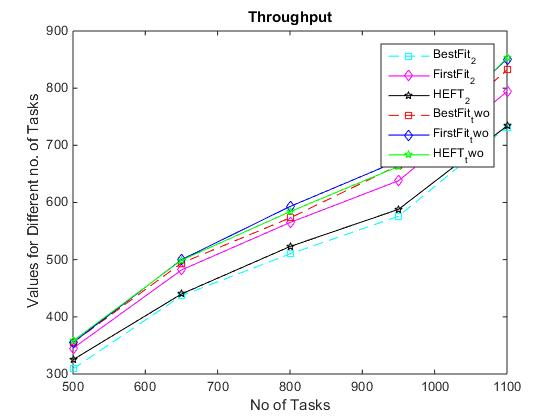
\includegraphics[scale=0.45]{tp_2_p.jpg}
\caption{TP2}
\label{fig}
\end{figure}

%\begin{figure}[htbp]
%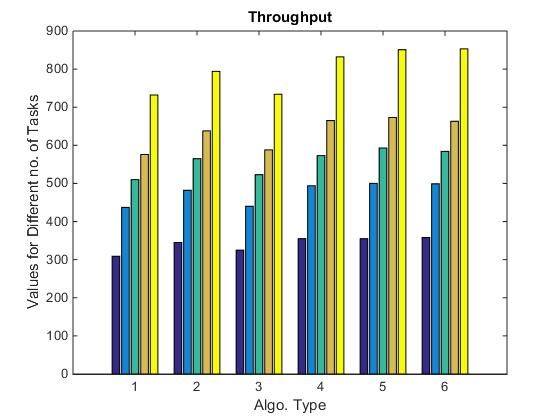
\includegraphics[scale=0.45]{tp_2_b.jpg}
%\caption{TP2}
%\label{fig}
%\end{figure}

\begin{figure}[htbp]
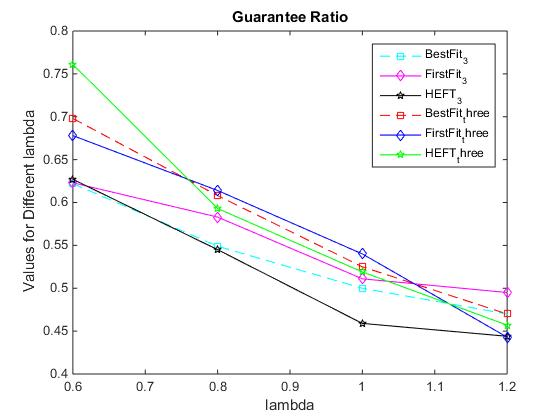
\includegraphics[scale=0.45]{gr_3_p.jpg}
\caption{GR3}
\label{fig}
\end{figure}

%\begin{figure}[htbp]
%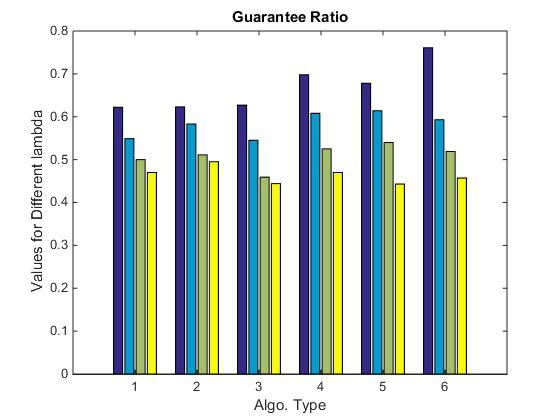
\includegraphics[scale=0.45]{gr_3_b.jpg}
%\caption{GR3}
%\label{fig}
%\end{figure}

\begin{figure}[htbp]
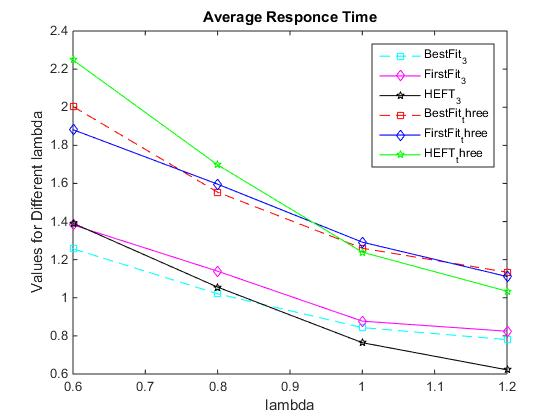
\includegraphics[scale=0.45]{art_3_p.jpg}
\caption{ART3}
\label{fig}
\end{figure}

%\begin{figure}[htbp]
%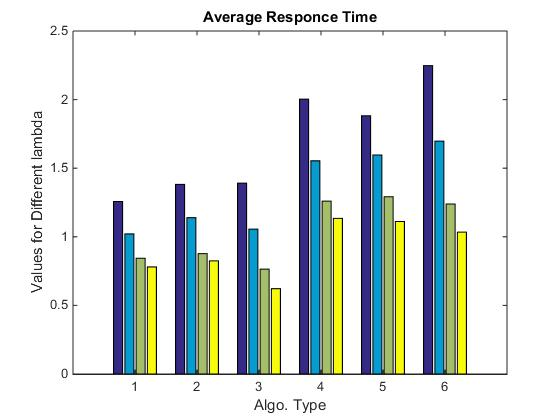
\includegraphics[scale=0.45]{art_3_b.jpg}
%\caption{ART3}
%\label{fig}
%\end{figure}

\begin{figure}[htbp]
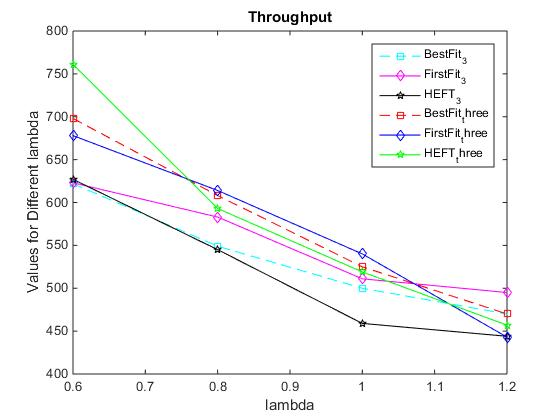
\includegraphics[scale=0.45]{tp_3_p.jpg}
\caption{TP3}
\label{fig}
\end{figure}

%\begin{figure}[htbp]
%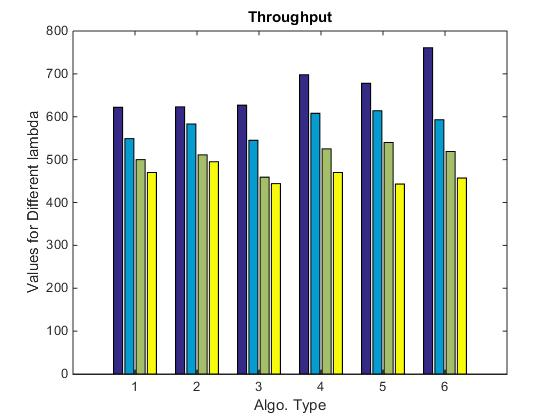
\includegraphics[scale=0.45]{tp_3_b.jpg}
%\caption{TP3}
%\label{fig}
%\end{figure}


\section{Conclusion}
The timing requirements of real-time task makes it difficult
to implement in cloud computing. It requires real-time virtualization technology for adoption of real-time applications. This paper presented three scheduling algorithms called BestFit, FirstFit, and HEFT where task are prioritised according to Deadline and Size. These algorithms performances are measured against BestFit EDF(BFE), FirstFit EDF(FFE) and HEFT(task prioritised according to deadline) algorithms. Different performance metrics used are Guarantee Ratio, Average Response Time, Throughput. Simulation results shows
that in all the cases proposed algorithms gives better results.


\begin{thebibliography}{11}
\bibitem{b1} Buyya, R., Yeo, C. S., Venugopal, S., Broberg, J., \& Brandic, I. (2009). Cloud computing and emerging IT platforms: Vision, hype, and reality for delivering computing as the 5th utility. Future Generation computer systems, 25(6), 599-616.
\bibitem{b2} Dastjerdi, A. V., Tabatabaei, S. G. H., \& Buyya, R. (2012). A dependency‐aware ontology‐based approach for deploying service level agreement monitoring services in Cloud. Software: Practice and Experience, 42(4), 501-518.
\bibitem{b3} Beloglazov, A., Abawajy, J., \& Buyya, R. (2012). Energy-aware resource allocation heuristics for efficient management of data centers for cloud computing. Future generation computer systems, 28(5), 755-768.
\bibitem{b4} An, K., Shekhar, S., Caglar, F., Gokhale, A., \& Sastry, S. (2014). A cloud middleware for assuring performance and high availability of soft real-time applications. Journal of Systems Architecture, 60(9), 757-769.
\bibitem{b5} Buttazzo, G. C. (2005). Rate monotonic vs. EDF: judgment day. Real-Time Systems, 29(1), 5-26.
\bibitem{b6} García-Valls, M., Cucinotta, T., \& Lu, C. (2014). Challenges in real-time virtualization and predictable cloud computing. Journal of Systems Architecture, 60(9), 726-740.
\bibitem{b7} Ekelin, C. (2006, July). Clairvoyant non-preemptive EDF scheduling. In null (pp. 23-32). IEEE.
\bibitem{b8} Liu, S., Quan, G., \& Ren, S. (2010, July). On-line scheduling of real-time services for cloud computing. In Services (SERVICES-1), 2010 6th World Congress on (pp. 459-464). IEEE.
\bibitem{b9} Shin, S., Kim, Y., \& Lee, S. (2015, January). Deadline-guaranteed scheduling algorithm with improved resource utilization for cloud computing. In Consumer Communications and Networking Conference (CCNC), 2015 12th Annual IEEE (pp. 814-819). IEEE.
\bibitem{b10} Lin, B., Guo, W., \& Lin, X. (2016). Online optimization scheduling for scientific workflows with deadline constraint on hybrid clouds. Concurrency and Computation: Practice and Experience, 28(11), 3079-3095.
\end{thebibliography}

\end{document}
